\section{Applications pratiques des suites}

\subsection{Les placements}

Sylvain dispose d'un capital de 10 000 €, qu'il place dans une banque. Cette banque lui propose un revenu fixe de 110 euros par mois. \\ On appelle $u_0$ le capital initial de Sylvain, et $u_n$ son capital au bout de $n$ mois. \\

Sylvette possède aussi un capital de 10 000 €, qu'elle place dans une autre banque. Elle les place à intérêts cumulés de 1 \% par mois. \\ On appelle $v_0$ le capital initial de Sylvette, et $v_n$ son capital au bout de $n$ mois. \\

\begin{itemize}
\item[1.]
\begin{itemize}
\item[a)] Calculer $u_1$ et $u_2$. Quel genre de suite est la suite $\left(u_n\right)_{n \in \N} $ ? \\
\item[b)] Calculer $v_1$ et $v_2$. Quel genre de suite est la suite $\left(v_n\right)_{n \in \N} $ ? \\
\end{itemize}
\item[2.]
\begin{itemize}
\item[a)] Sylvain et Sylvette décident tous les deux de placer leur capital pendant un an. Lequel des deux a fait le meilleur choix ? \\
\item[b)] Sylvain et Sylvette décident tous les deux de placer leur capital pendant deux ans. Lequel des deux a fait le meilleur choix ? \\
\end{itemize}
\item[3.] 
\begin{itemize}
\item[a)] Au bout de combien de mois le capital de Sylvain aura-t-il doublé ?
\item[b)] Au bout de combien de mois le capital de Sylvette aura-t-il doublé ?
\end{itemize} 
\end{itemize}

\vspace*{.3cm}

\begin{itemize}
\item[1.]
\begin{itemize}
\item[a)] 
\begin{itemize}
\item[•] $u_0 = 10 000$ \\
\item[•] $u_1 = u_0 + 110 = 10 000 + 110 = 10110$ \\
\item[•] $u_2 = u_1 + 110 = 10110 + 110 = 10220$ \\
\end{itemize}
\vspace*{.3cm}
$\left(u_n\right)_{n \in \N}$ est une suite arithmétique de premier terme $u_0 = 10 000$ et de raison $r = 110$. \\

\begin{tabular}{lllll}
Donc, on a & $\forall n \in \N$, & $ u_n $ & $ = $ &$ u_0 + nr$ \\
& $\forall n \in \N$, & $u_n $ & $=$ & $10 000 + 110n$ \vspace*{.3cm} \\
\end{tabular}
\item[b)] 
\begin{itemize}
\item[•] $v_0 = 10 000$ \\
\item[•] $v_1 = v_0 \times 1,01 = 10 000 \times 1,01 = 10100$ \\
\item[•] $v_2 = v_1 \times 1,01 = 10 100 \times 1,01 = 10201$ \\
\end{itemize}
\vspace*{.3cm}
$\left(v_n\right)_{n \in \N}$ est une suite géométrique de premier terme $u_0 = 10 000$ et de raison $q = 1,01$. \\

\begin{tabular}{lllll}
Donc, on a & $\forall n \in \N$, & $ v_n $ & $ = $ &$ u_0 \times q^n$ \\
& $\forall n \in \N$, & $v_n $ & $=$ & $10 000 \times 1,01^n$ \vspace*{.3cm} \\
\end{tabular}
\end{itemize}
\end{itemize}

\newpage

\begin{itemize}
\item[2.]
\begin{itemize}
\item[a)]
\begin{itemize}
\item[*] Sylvain place son argent 12 mois, on calcule donc $u_{12}$. \\

On a $u_{12} = \left(110 \times 12\right) + 10 000$ \\

Donc $u_{12} = 11320$ \\

\item[*] Sylvette place aussi son argent 12 mois, on calcule donc $v_{12}$ \\

On a $v_{12} = 10 000 \times 1,01^{12}$ \\

Donc $v_{12} \approx 11 268,25$ \\

Donc Sylvain a fait un meilleur choix. \\
\end{itemize}
\item[b)] 
\begin{itemize}
\item[*] Sylvain place son argent 24 mois, on calcule donc $u_{24}$. \\

On a $u_{24} = \left(110 \times 24\right) + 10 000$ \\

Donc $u_{24} = 12640$ \\

\item[*] Sylvette place aussi son argent 24 mois, on calcule donc $v_{24}$ \\

On a $v_{24} = 10 000 \times 1,01^{24}$ \\

Donc $v_{24} \approx 12 697,35$ \\

Donc Sylvette a fait un meilleur choix. \\
\end{itemize}
\item[3.] 
\begin{itemize}
\item[a)] On cherche $u_n \geqslant 20 000$ \\

\begin{tabular}{rll}
$u_n$ & $ \geqslant $ & $ 20 000$ \\
$10 000 + 110n$ & $\geq$ & $20 000$ \\
$110n$ & $\geq$ & $10 000$ \\
$n$ & $\geq$ & $\dfrac{10 000}{110}$ \\
$n$ & $\geq$ & $90,9$ \\
$n$ & $\geq$ & $91$ \vspace*{.3cm}\\
\end{tabular} 

Donc le capital de Sylvain aura doublé au bout de 91 mois. \\

\item[b)] On cherche $v_n \geqslant 20 000$ \\
\begin{tabular}{rll}
$u_n$ & $ \geqslant $ & $ 20 000$ \\
$10 000 \times 1,01^n$ & $\geq$ & $20 000$ \\
$1,01^n$ & $\geq$ & $2$ \vspace*{.3cm} \\
\end{tabular} 

La plus petite valeur possible de $n$ telle que $1,01^n \geqslant 2$ est $70$. \\

Donc le capital de Sylvette aura doublé au bout de 70 mois.
\end{itemize}
\end{itemize}
\end{itemize}

\newpage

\vspace*{-.5cm}

\subsection{Les emprunts}

\textbf{Exercice} \\

On appelle $k$ le capital emprunté, et donc à rembourser. Les versements ($v$) sont constitués de :

\begin{itemize}
\item[1.] Les amortissements ($a$) : c'est la partie du capital que l'on rembourse.
\item[2.] les intérêts ($i$). 
\end{itemize}

On a donc $v = a + i$. \\

1) Soit un emprunt à amortissement constant d'un capital $k = 20 000$ €. Le taux d'intérêt annuel est de 12 \%. Il faut rembourser le capital en 4 versements annuels. \\

On a : \\

\begin{tabular}{|c|c|c|c|c|}
\hline
Période & Capital dû restant & intérêts & amortissements & versements \\
\hline
Fin de la 1$^{\mathrm{ère}}$ année & 20 000 & 2400 & 5000 & 7400 \\
\hline
Fin de la 2$^{\mathrm{ème}}$ année & 15 000 & 1800 & 5000 & 6800 \\
\hline
Fin de la 3$^{\mathrm{ème}}$ année & 10 000 &  1200 & 5000 & 6200 \\
\hline
Fin de la 4$^{\mathrm{ème}}$ année & 5 000 & 600 & 5000 & 5600 \\
\hline
\end{tabular}

\vspace*{.3cm}

Les versements forment une suite arithmétique $\left(v_n\right)_{n\in \N^*}$ de raison $r = -600$. \\

\begin{tabular}{lll}
$v_n$ & $ = $ & $ v_1 - \left(n-1\right)r$ \\
& $=$ & $7400 - 600\left(n-1\right)$ \\
& $=$ & $8000 - 600n$ \\
\end{tabular}

\vspace*{.3cm}

On a bien $v_4 = 8000 - 600 \times 4 = 8000 - 2400 = 5600$ \\

Calculons le coup du crédit : \\

\begin{tabular}{rll}
On a : $S$ & $=$ & $v_1 + v_2 + v_3 + v_4$ \vspace*{.3cm} \\
& $=$ & $n \dfrac{v_1 + v_4}{2}$ \vspace*{.3cm} \\
& $=$ & $4 \times \dfrac{7400 + 5600}{2}$ \vspace*{.3cm} \\
& $=$ & $26000$ \\
\end{tabular}

\vspace*{.3cm}

On a donc $30$ \% d'intérêts. \\

2) Soit un emprunt à versements constants d'un capital $k = 10 000$ €. Le taux d'intérêt annuel est de 15 \%. Il faut rembourser le capital en 3 versements annuels. \\

On a : \\

\begin{tabular}{|c|c|c|c|c|}
\hline
Période & Capital dû restant & intérêts & amortissements & versements \\
\hline
Fin de la 1$^{\mathrm{ère}}$ année & 10 000 & 1500 & $a_1 = 2879,77$ & $v = 4379,77$ \\
\hline
Fin de la 2$^{\mathrm{ème}}$ année & $10000 - a_1$ & 1068 & $a_2 = 3311,74$ & $v = 4379,77$ \\
& $= 7120,33$ & & & \\
\hline
Fin de la 3$^{\mathrm{ème}}$ année & $ 7120,23 - 3311,74$ & $571,27$ & $a_3 = 3808,5$ & $v = 4379,77$ \\
& $3808,49$ & & & \\
\hline
\end{tabular}

\newpage

\vspace*{-.5cm}

$v = a_1 + 0,15k$ pour le premier versement. \\

$v = a_2 + 0,15\left(k-a_1\right)$ pour le deuxième versement. \\

\begin{tabular}{lrll}
D'où & $a_2 + 0,15\left(k - a_1\right) $ & $=$ & $a_1 + 0,15k$ \\
& $a_2 + 0,15k - 0,15a_1$ & $ = $ & $ a_1 + 0,15k$ \\
& $a_2 - 0,15a_1$ & $ = $ & $ a_1$ \\
& $a_2$ & $=$ & $a_1 \left(1 + 0,15\right)$ \\
& $a_2$ & $=$ & $a_1 \times 1,15$ \\
\end{tabular}

\vspace*{.3cm}

De même, $v = a_2 + 0,15\left(k-a_1\right)$ pour le deuxième versement, et $v = a_3 + 0,15\left(k - a_1 - a_2\right)$ pour le troisième versement. \\

\begin{tabular}{lrll}
D'où & $a_3 + 0,15\left(k - a_1 - a_2\right)$ & $=$ & $a_2 + 0,15\left(k-a_1\right)$ \\
& $a_3 + 0,15k - 0,15a_1 - 0,15a_2$ & $ = $ & $ a_2 + 0,15k - 0,15a_1$ \\
& $a_3 - 0,15a_2$ & $ = $ & $ a_2$ \\
& $a_3$ & $=$ & $a_2 \left(1 + 0,15\right)$ \\
& $a_3$ & $=$ & $a_2 \times 1,15$ \\
\end{tabular}

\vspace*{.3cm}

Les versements forment une suite géométrique $\left(v_n\right)_{n \in \N^*}$ de raison $q = 1,15$ \\

Or, $a_1 + a_2 + a_3 = 10 000$ \\

Donc $a_1 \times \dfrac{1-q^n}{1-q} = 10000$\\

$a_1 \times \dfrac{1-1,15^3}{1 - 1,15} = 10 000$ \\

Il vient que $a_1 = 10 000 \dfrac{1-1,15}{1-1,15^3}$ et$a_1 \approx 2879,77$ \\

Le coût du crédit est de $3v = 13 139,31$ €, soit $31,4$\%. \\

\textbf{Amusette} \\

Sylvain emprunte $1000$ € pendant 1 an. Son remboursement se fait par un versement unique à taux 6,62 \% annuel. \\

Sylvette emprunte $1 000$ € pendant 1 an. Son remboursement se fait par douze versements à taux \\ 1 \% mensuel. \\

Combien Sylvain doit-il payer pour rembourser son emprunt ? Et combien Sylvette doit-elle payer pour rembourser son emprunt ? \\ 

\begin{itemize}
\item[•] \textbf{Sylvain} : il rembourse à un taux de 6,62 \%, il paiera donc : $1000 \times 1,0662 = 1066,2$ €. \\
\item[•] \textbf{Sylvette} : dans son cas, les amortissements forment une suite géométrique $\left(a_n\right)_{n\in \N^*}$ de raison $q = 1,01$. \\

Or, on a $a_1 + a_2 + a_3 + ... + a_{12} = 1000$. D'où $a_1 \times \dfrac{1-1,01^{12}}{1-1,01} = 1000$ \\

Donc $a_1 \approx 78,85$.

%Partie à compléter... Pas d'information supplémentaire dans les cahiers des élèves... Essayer de trouver un 3e cours ? Cécile ? 
\end{itemize}

\newpage

\vspace*{-1cm}

\subsection{Exercice : À la montagne...}

Le conseil municipal d'une station touristique de montagne a décidé de faire équiper une falaise afin de créer un site d'escalade. L'équipement doit se faire depuis le pied de la falaise. Deux entreprises spécialisées dans ce type de chantier ont été contactées et ont envoyé des devis. On se propose d'étudier ceux-ci : \\

\begin{itemize}
\item[•] \textbf{Devis A} : Le premier mètre équipé coûte 100 € puis chaque mètre supplémentaire équipé coûte 20 € de plus que le mètre précédent (100 € pour équiper une falaise d'un mètre, $100 + 120 = 220$ € pour équiper une falaise de deux mètres, $100 + 120 + 140 = 360$ pour équiper une falaise de trois mètres, etc.) \\
\item[•] \textbf{Devis B} : Le premier mètre équipé coûte 50 € puis chaque mètre supplémentaire équipé coûte 5\% de plus que le mètre précédent (50 € pour équiper une falaise d'un mètre, $50 + 52,50 = 102,50$ € pour équiper une falaise de deux mètres, $50 + 52,50 + 55,215 = 157,625$ € pour équiper une falaise de trois mètres, etc.) \\
\end{itemize}

On appelle $u_n$ le prix d'un n-ième mètre équipé et $S_n$ le prix de l'équipement d'une falaise de $n$ mètres de hauteur indiqué par l'entreprise A. \\
On appelle $v_n$ le prix d'un n-ième mètre équipé et $R_n$ le prix de l'équipement d'une falaise de $n$ mètres de hauteur indiqué par l'entreprise B. \\

\begin{itemize}
\item[1.] Exprimer $u_n$ et $S_n$ en fonction de $n$. \\
\item[2.] Exprimer $v_n$ et $R_n$ en fonction de $n$. \\
\item[3.] Calculer le prix à payer pour équiper une falaise de 92 mètres de hauteur avec chacune des deux entreprises. Préciser l'entreprise la moins chère. On arrondira les prix à l'euro près. \\
\item[4.] Le conseil municipal a décidé d'accorder un budget de 120 000 € pour équiper le site. Calculer la hauteur de la falaise qui peut être équipée avec cette \hbox{somme par chacune des deux entreprises A et B} (on arrondira les hauteurs au mètre près). \\
\end{itemize}

\vspace*{.3cm}

\begin{itemize}
\item[1.] Soit $\left(u_n\right)_{n\in \N^*}$ la suite arithmétique de premier terme $u_1 = 100$ et de raison $r = 20$ \\

\begin{tabular}{rrll}
On a $\forall n \in \N^*$, & $u_n$ & $ =$ & $ u_1 + \left(n-1\right)r$ \\
& $u_n$ & $=$ & $100 + 20\left(n-1\right)$ \\
Donc & $u_n$ & $=$ & $80 + 20n$ \\
\end{tabular}

\vspace*{.3cm} 

\begin{tabular}{rrll}
On a $\forall n \in \N^*$, & $S_n$ & $ = $ & $ n \dfrac{u_1 + u_n}{2}$ \vspace*{.3cm} \\
& $S_n$ & $=$ & $n \dfrac{100 + 80 + 20n}{2}$ \vspace*{.3cm} \\
& $S_n$ & $=$ & $n \dfrac{180 + 20n}{2}$ \vspace*{.3cm} \\
& $S_n$ & $=$ & $n \dfrac{2\left(10n + 90\right)}{2}$ \vspace*{.3cm} \\
& $S_n$ & $=$ & $n\left(10n + 90\right)$ \vspace*{.3cm} \\
Donc & $S_n$ & $=$ & $10n^2 + 90$
\end{tabular}

\vspace*{-5cm}

\end{itemize}

\newpage

\begin{itemize}
\item[2.] Soit $\left(v_n\right)_{n\in \N^*}$ la suite géométrique de premier terme $v_1 = 50$ et de raison $r = 1,05$ \\

\begin{tabular}{rrll}
On a $\forall n \in \N^*$, & $v_n$ & $ =$ & $ v_1 \times q^{n-1}$ \\
Donc & $v_n$ & $=$ & $50 \times \left(1,05\right)^{n-1}$ \\
\end{tabular}

\vspace*{.3cm} 

\begin{tabular}{rrll}
On a $\forall n \in \N^*$, & $R_n$ & $ = $ & $ v_1\times \dfrac{1-q^n}{1-q}$ \vspace*{.3cm} \\
& $R_n$ & $=$ & $50 \times \dfrac{1-\left(1,05\right)^{n}}{1- 1,05}$ \vspace*{.3cm} \\
Donc & $R_n$ & $=$ & $-1000\left[1 - \left(1,05\right)^n\right]$ \vspace*{.3cm} \\
\end{tabular}

\item[3.] On cherche $S_{92}$. On calcule $u_{92} = u_1 + \left(92-1\right)r = 100 + 91\times 20 = 1920$ \\

On a donc : $92 \times \dfrac{100 + 1920}{2}$

D'où $S_{92} = 92920$ \\

On cherche ensuite $R_{92}$. \\

On a donc : $u_1 \times \dfrac{1 - q^{92}}{1 - 1,05} = 50 \times \dfrac{1-1,05^{92}}{1-1,05} \approx 88005$ \\

D'où $R_{92} = 88005$. On préfèrera choisir l'entreprise B. \\

\item[4.] On cherche $S_n \leqslant 120 000$ \\

\begin{tabular}{rll}
$10n^2 + 90n$ & $ \leqslant $ & $ 120 000$ \\
$10n^2 + 90n - 120 000$ & $ \leqslant $ & $0$ \\
\end{tabular}

\vspace*{.3cm}

On a $n_1 \approx -114,1$ et $n_2 \approx 105,1$ \\

\begin{tikzpicture}
\tkzTabInit[lgt=4.2,espcl=3]
{ $n$  /1,
$10n^2 + 90n - 120 000$ /1}
{$ - \infty $ , $n_1$, $0$ , $n_2$,  $ + \infty $}
\tkzTabLine{ , +, z, -, t, -, z, + }
\end{tikzpicture}

\vspace*{.3cm}

On sait que $n \geqslant 0$. On peut donc équiper une mur d'une hauteur compris entre 0 et 105 mètres avec une subvention de $120 000$ €. \\

On cherche $R_n \leqslant 120 000$ \\

\begin{tabular}{rll}
$ -1000\left[1-\left(1,05\right)^n\right]$ & $\leq$ &  $120 000$ \\
$1-\left(1,05\right)^n$ & $\geq$ & $-120$ \\
$-\left(1,05\right)^n$ & $\geq$ & $-121$ \\
$\left(1,05\right)^n$ & $\leq$ & $121$ \\
\end{tabular}

\vspace*{.3cm}

On peut donc équiper un mur d'une hauteur maximale de 98 mètres. On préfèrera choisir le devis A pour les travaux.

\end{itemize}

\newpage

\vspace*{-1.7cm}

\section{Deux exemples de suites arithmético-géométriques}

\subsection{Exemple \no 1}

Soit $\left(u_n\right)_{n \in \N}$ la suite définie par :$ \; \; \; \begin{cases}
u_0 = 10 \\
\forall n \in \N, u_{n+1} = \dfrac{1}{2} u_n - 3 \\
\end{cases}$ \\

\begin{itemize}
\item[1.] Déterminer $u_1$, $u_2$, $u_3$ et $u_4$. 
\item[2.] Soit $\left(v_n\right)_{n \in \N}$ la suite définie par $v_n = u_n + 6$. Montrer que $\left(v_n\right)_{v \in \N}$ est une suite géométrique dont on déterminera le premier terme et la raison. 
\item[3.] Exprimer $v_n$ en fonction de $n$, puis $u_n$ en fonction de $n$. 
\item[4.]  Déterminer $\lim\limits_{n \to +\infty} v_n$ puis $\lim\limits_{n \to +\infty} u_n$ \\
\end{itemize}

\begin{itemize}
\item[1.]
\begin{itemize}
\item[•] $u_0 = 10$ \\
\item[•] $u_1 = \dfrac{1}{2} u_0 - 3 = 5 - 3 = 2$ \\
\item[•] $u_2 = \dfrac{1}{2} u_1 - 3 = 1 - 3 = -2$ \\
\item[•] $u_3 = \dfrac{1}{2} u_2 - 3 = -1 - 3 = -4$ \\
\item[•] $u_4 = \dfrac{1}{2} u_3 - 3 = -2 - 3 = -5$ \\
\end{itemize}
\item[2.] Étudions $v_{n+1}$ \\
\begin{tabular}{lll}
$v_{n+1}$ & $=$ & $u_{n+1} + 6$ \vspace*{.3cm} \\
& $=$ & $\left(\dfrac{1}{2}u_n - 3\right)+6$ \vspace*{.3cm} \\
& $=$ & $\dfrac{1}{2}u_n + 3$ \vspace*{.3cm} \\
& $=$ & $\dfrac{1}{2} \left(v_n - 6\right) + 3$ \vspace*{.3cm} \\
& $=$ & $\dfrac{1}{2} v_n - 3 + 3$ \vspace*{.3cm} \\
& $=$ & $\dfrac{1}{2} v_n$ \\
\end{tabular}
\vspace*{.3cm}

Donc $\left(v_n\right)_{v \in \N}$ est une suite géométrique de premier terme $v_0 = u_0 + 6 = 10 + 6 = 16$ et \\ de raison $q = \dfrac{1}{2}$ \vspace*{.3cm} \\

\item[3.] On $v_n = v_0 \times q^n$, donc $v_n = 16 \times \left(\dfrac{1}{2}\right)^n$ \\

On a $u_n = v_n - 6$, donc $u_n = 16 \times \left(\dfrac{1}{2}\right)^n - 6$ \\

Donc $\forall n \in \N, u_n = 16 \times \left(\dfrac{1}{2}\right)^n - 6$ \\

\item[4.] $\lim\limits_{n \to +\infty} v_n = 0$, car $\left(v_n\right)_{n \in \N}$ est une suite géométrique de raison $q = \dfrac{1}{2}$, et $ 0 < q < 1$ \\

$\lim\limits_{n \to +\infty} u_n = -6$, car $u_n = v_n - 6$ 
\end{itemize}

\vspace*{-5cm}

\newpage

\subsection{Exemple \no 2}

Soit $\left(u_n\right)_{n \in \N}$ la suite définie par :$ \; \; \; \begin{cases}
u_0 = 10 \\
\forall n \in \N, u_{n+1} = -\dfrac{1}{2} u_n + 3 \\
\end{cases}$ \\

\begin{itemize}
\item[1.] Déterminer $u_1$, $u_2$, $u_3$ et $u_4$. 
\item[2.] Soit $\left(v_n\right)_{n \in \N}$ la suite définie par $v_n = u_n - 2$. Montrer que $\left(v_n\right)_{v \in \N}$ est une suite géométrique dont on déterminera le premier terme et la raison. 
\item[3.] Exprimer $v_n$ en fonction de $n$, puis $u_n$ en fonction de $n$. 
\item[4.]  Déterminer $\lim\limits_{n \to +\infty} v_n$ puis $\lim\limits_{n \to +\infty} u_n$ \\
\end{itemize}

\begin{itemize}
\item[1.]
\begin{itemize}
\item[•] $u_0 = 10$ \\
\item[•] $u_1 = -\dfrac{1}{2} u_0 + 3 = -5 + 3 = -2$ \\
\item[•] $u_2 = -\dfrac{1}{2} u_1 + 3 = 1 + 3 = 4$ \\
\item[•] $u_3 = -\dfrac{1}{2} u_2 + 3 = -2 + 3 = 1$ \\
\item[•] $u_4 = -\dfrac{1}{2} u_3 + 3 = -\dfrac{1}{2} + 3 = \dfrac{5}{2}$ \\
\end{itemize}
\item[2.] Étudions $v_{n+1}$ \\
\begin{tabular}{lll}
$v_{n+1}$ & $=$ & $u_{n+1} -2$ \vspace*{.3cm} \\
& $=$ & $\left(-\dfrac{1}{2}u_n + 3\right)-2$ \vspace*{.3cm} \\
& $=$ & $-\dfrac{1}{2}u_n +1$ \vspace*{.3cm} \\
& $=$ & $-\dfrac{1}{2} \left(v_n + 2\right) + 1$ \vspace*{.3cm} \\
& $=$ & $-\dfrac{1}{2} v_n - 1 + 1$ \vspace*{.3cm} \\
& $=$ & $-\dfrac{1}{2} v_n$ \\
\end{tabular}
\vspace*{.3cm}

Donc $\left(v_n\right)_{v \in \N}$ est une suite géométrique de premier terme $v_0 = u_0 - 2 = 10 - 2 = 8$ et \\ de raison $q = -\dfrac{1}{2}$ \vspace*{.3cm} \\

\item[3.] On $v_n = v_0 \times q^n$, donc $v_n = 8 \times \left(-\dfrac{1}{2}\right)^n$ \\

On a $u_n = v_n + 2$, donc $u_n = 8 \times \left(-\dfrac{1}{2}\right)^n + 2$ \\

Donc $\forall n \in \N, u_n = 8 \times \left(-\dfrac{1}{2}\right)^n + 2$ \\

\item[4.] $\lim\limits_{n \to +\infty} v_n = 0$, car $\left(v_n\right)_{n \in \N}$ est une suite géométrique de raison $q = -\dfrac{1}{2}$, et $ -1 < q < 0$ \\

$\lim\limits_{n \to +\infty} u_n = 2$, car $u_n = v_n + 2$ 
\end{itemize}

\vspace*{-5cm}